\documentclass[12pt,a4paper]{article}

\usepackage{amssymb}
\usepackage{amsthm}
\usepackage[scale=0.75]{geometry} 
\usepackage[pagebackref=true,colorlinks,linkcolor=blue,citecolor=magenta]{hyperref}
\usepackage{tocbibind}
\usepackage{ragged2e}
\usepackage{xepersian}

\settextfont[Scale=1]{XB Niloofar}
\setlatintextfont{Linux Libertine}

\setlength{\parskip}{1em}
\renewcommand{\baselinestretch}{1.5}

\theoremstyle{definition}
\newtheorem{exmp}{مثال}[section]

\title{‌سیستم‌های فازی و هوش مصنوعی}
\author{کاوه شاه‌حسینی}

\begin{document}
%*******************Cover Page****************************
\thispagestyle{empty}
\vspace*{-28mm}
\centerline{
\includegraphics[height=4cm]{pnu-logo.jpg}}
\begin{center}
	\vspace{-2mm}
	{\large
	دانشگاه پیام نور تهران مرکز شمیرانات
	\\[.1cm]
	دانشکده مهندسی کامپیوتر
	\\[.1cm]
		مهندسی نرم‌افزار
	\\[1.7cm]
		عنوان سمینار
	\\[.9cm]
	}
	{\Huge 
		سیستم‌های فازی و هوش مصنوعی
	}
	\\[1.8cm]
	استاد 
	\\[.2cm]
	\textbf{\large {دکتر مهدی خلیلی}}
	\\[1.5cm]
	دانشجو
	\\[.1cm]
	\textbf{\large { کاوه شاه‌حسینی}}
	\\[1.5cm]
	شماره دانشجویی
	\\[.1cm]
	\textbf{\large {۹۲۳۸۴۳۰۱۰‌}}
	\\[1.5cm]
	{\large
		ترم ۳۹۵۱
	}
\end{center}
%********************Table of Content**********************
\newpage
\baselineskip=1cm
\tableofcontents
\newpage
\listoftables
\baselineskip=.75cm
\newpage 
%*******************Fuzzy Sets****************************
\section{مجموعه‌های فازی}
 \subsection{مجموعه‌های کلاسیک}
پیش از آنکه به توضیح مجموعه‌های فازی بپردازیم، نیاز است تا مروری بر مجموعه‌های کلاسیک داشته باشیم. همه‌ی ما کم و بیش با مفهموم مجموعه آشنا هستیم. به عنوان مثال مجموعه‌ای از دانشجویان یک رشته، مجموعه‌ای از اعداد بزرگ‌تر از صفر و... نمونه‌ای از مجموعه‌ها هستند. مجموعه‌ها گروهی از اشیاء متمایز هستند. به اشیاء درون هر مجموعه، اعضاء و یا عناصر آن مجموعه گفته می‌شود. \\
در ریاضیات مجموعه را با حروف بزرگ 
$\lr{A,B,C,...}$
 و اعضای مجموعه را با حروف کوچک 
$\lr{a,b,c,...} $
  نمایش می‌دهند. همچنین عضویت یک شیء در مجموعه با نماد 
$\in$
 و عدم عضویت با نماد
 $\notin$
 نمایش داده می‌شود. 
 \cite{Bojadziev2007}
 \\
مجموعه‌ای را که شامل همه‌ی اشیاء در یک کاربرد مشخص هستند را مجموعه‌ی جهانی 
\LTRfootnote{Universal Set}
یا مرجع گویند. \\
اگر مجموعه‌ی جهانی را با $ U $  نمایش دهیم، آنگاه نمایش مجموعه‌ی $ A $  در این مجموعه‌ی مرجع می‌تواند به دو روش صورت گیرد. در روش اول می‌توان تمامی عناصر موجود در مجموعه را با لیست کردن 
\LTRfootnote{Listing Method}
نمایش داد. به عنوان مثال اگر مجموعه‌ی $ A $ مجموعه‌ی اعداد طبیعی کوچک‌تر از ۵ باشد، می‌توان آن را به صورت زیر نمایش داد.
\begin{equation}
A=\{1,\ 2,\ 3,\ 4\}
\end{equation}
و یا می‌توان با استفاده از روش دوم یعنی قانون عضویت
\LTRfootnote{Membership Rule}
بصورت زیر نمایش داد.
\cite{Wang1997}
\begin{equation}
 A= \{ x\ |\ x \in N,\ x < 5\} 
 \end{equation}
 روش دوم به این صورت خوانده می‌شود «مجموعه‌ی $ A $، شامل اعضای $ x $ است، به قسمی که  $ x $ها جزو اعداد طبیعی باشند و کوچک‌تر از ۵ باشند».\\
 به صورت کلی تعریف مجموعه‌ها با استفاده از قوانین عضویت به صورت زیر نوشته می‌شود:
\begin{equation}
 A= \{  x \in U\ |\   x\ {\rm meets\ some\ conditions } \}
 \end{equation} 
 در مجموعه‌های کلاسیک عضویت یک شیء تنها دو حالت دارد بدین صورت که شیء $x$ یا متعلق به مجموعه $A$ هست و یا نیست. این مجموعه‌ها را به دلیل آنکه فضای آن با دقت ۱۰۰٪ قابل تشخیص است و عناصر آن دارای ارزش عضویت صفر و یا یک هستند، مجموعه‌های
  \textbf{قطعی}
  نیز می‌گویند. 
\begin{equation}\label{f_2}
\mu_{A}(x)=\left \{ 
	{1 \atop 0}
	\hskip 1cm
   {if \hskip 1cm x \in A, \atop
	if \hskip 1cm x \notin A.} \right.
\end{equation} 
در اینجا
$\mu_{A}(x)$
 تابع عضویت مجموعه‌ی قطعی $A$ می‌باشد. تابع عضویت، تابعی است که ارزش عضویت یک شیء را در یک مجموعه، مشخص می‌کند. طبق آنچه در رابطه
 \ref{f_2}
 آمده است، تابع عضویت مجموعه‌های قطعی، تنها دو مقدار یک و یا صفر را برای مشخص کردن عضویت و یا عدم عضویت یک شیء در مجموعه، بازمی‌گرداند. تابع عضویت مجموعه‌ی جهانی همواره مقدار یک (۱) را بازمی‌گرداند. همچنین اگر مجموعه‌ای دارای هیچ عضوی نباشد، آن مجموعه‌ را تهی
 \LTRfootnote{Empty Set}
 می‌نامند و با علامت $\varnothing$ نمایش داده می‌شود. مجموعه‌ی تهی زیرمجموعه‌ی هر مجموعه‌ای است.
 \cite{Lee2005}
 \\
فرض کنید دو مجموعه‌ی $ A $ و $ B  $ در مجموعه‌ی مرجع $ U $ وجود دارد.  در جدول   
\ref{table:t_1}
\textbf{روابط بین مجموعه‌های کلاسیک} 
 همراه با توضیح آورده شده است:
\begin{table}[!htbp]
\begin{center}
	{\footnotesize
 \begin{tabular}{r c c r} \hline
عنوان & نماد &  مثال & توضیح  
\\\hline 
%**********
زیر مجموعه  &
$\subseteq$ &
$A \subseteq B$ &
همه‌ی اعضای $A$ در $B$ نیز هست و یا دو مجموعه با یکدیگر مساوی هستند.
\\
%*********
زیر مجموعه سره &
$\subset$ &
 $A \subset B$ &
همه‌ی اعضای $A$ در $B$ نیز هست. ولی حداقل یک عضو در $B$ هست که در $A$ نیست.
\\
%**********
مساوی &
$=$ &
$A = B$ &
همه‌ی اعضای $A$ در $B$ نیز هست و همه‌ی اعضای $B$ نیز در $A$ هست.
\\\hline
 %**********
 \end{tabular}
 \caption{روابط بین مجموعه‌های کلاسیک}
 \label{table:t_1}
}
\end{center}
\end{table}
\\
همچنین در جدول
\ref{table:t_2}
\textbf{عملیات بر روی مجموعه‌های کلاسیک} 
همراه با تعاریف هریک از آنها آورده شده‌ است:
\begin{table}[!htbp]
	{\footnotesize
	\begin{center}
		\begin{tabular}{r c l} \hline
			عنوان & نماد & تعریف  
			\\\hline 
			%**********
			اجتماع   &
			$\cup$ &
			$A \cup B = \{x\ |\ x \in A\ {\rm or}\ x \in B \}$ 
			\\
			%*********
			اشتراک   &
			$\cap$ &
			$A \cap B = \{x\ |\ x \in A\ {\rm and}\ x \in B \}$ 
			\\
			%**********
			تفاضل &
			$-$ &
			$A - B = \{x\ |\ x \in A\ {\rm and}\ x \notin B \}$ 
		   \\
			%**********
			مکمل &
			$\overline{A}$ &
			$\overline{A} = \{x\ |\ x \notin A{\rm ,}\ x \in U \}$ 
			\\\hline 
			%**********
		\end{tabular}
		\caption{عملیات بر روی مجموعه‌های کلاسیک}
		\label{table:t_2}
\end{center}
	}
\end{table} 
\\

%***************************************************************************
 \subsection{تعریف مجموعه‌های فازی}
 
%##################################################################
در سال ۱۹۶۵ پروفسور لطفی‌زاده، مفهوم عضویت درجه‌بندی شده و غیردقیق را مطرح کرد. در این روش درجه عضویت اعضای یک مجموعه مانند مجموعه‌های قطعی محدود به صفر و یک نمی‌شود و می‌تواند شامل درجات عضویت بین صفر تا یک نیز باشد. لطفی‌زاده این مجموعه‌ها را 
\textbf{مجموعه‌های فازی}
\LTRfootnote{Fuzzy Sets}
 نامید. مفهوم کلمه‌ی فازی به معنای نادقیق و مبهم می‌باشد. \\
 مجموعه‌های کلاسیک را می‌توان به عنوان نمونه‌ی خاصی از مجموعه‌های فازی درنظر گرفت که تمامی اعضای آن دارای درجه عضویت یک می‌باشند.
 \cite{Bojadziev2007}
 \\
 در برخی موارد برای تمایز بین مجموعه‌های کلاسیک و فازی، از علامت $\widetilde{A}$ استفاده می‌شود. 
 \cite{Lee2005}
 در اینجا ما برای راحتی، از علامت $ \sim $ بر روی نام مجموعه‌های فازی استفاده نمی‌کنیم.
 \\
 اگر مجموعه‌ی $A$ را در مجموعه‌ی مرجع $U$، یک مجموعه فازی درنظر بگیریم، آنگاه $A$ به صورت زیر تعریف می‌شود:
\begin{equation}\label{f_3}
A= \{  (x, \mu_{A}(x))\ |\ x \in A, \mu_{A}(x) \in [0,1]  \}
\end{equation} 
که در آن $\mu_{A}(x)$ تابع عضویت مجموعه‌ی $A$ می‌باشد و برای هر عضو درجه‌ی عضویت آن را مشخص می‌کند. 
در برخی منابع تعریف مجموعه‌ی فازی به صورت زیر نیز آورده شده است:
\begin{equation}\label{f_4}
A= \{  \mu_{A}(x)/x \ |\ x \in A, \mu_{A}(x) \in [0,1]  \}
\end{equation} 
در راین رابطه علامت $/$ به معنی تقسیم نیست، بلکه روشی دیگر برای نمایش اعضای مجموعه است که در آن، عدد بالای این نماد درجه عضویت و عدد زیرین عضو مجموعه می‌باشد.
 \cite{Bojadziev2007}
 \\
برای \textbf{نمایش مجموعه‌های فازی} می‌توان طبق رابطه
\ref{f_3}
لیست زوج مرتبی از عناصر مجموعه و درجه عضویت آنها را نمایش داد. به عنوان مثال فرض کنید عناصر 
$ x_{i}=1,2,...,5 $
متعلق به مجموعه‌ی $A$ هستند و به ترتیب دارای درجات عضویت 
$1, 0.8, 0.3, 0.5, 0.1$
می‌باشند. این مجموعه فازی را می‌توان به صورت:
\begin{equation}
A = \{ ( 1, 0.1), (2, 0.5), (3, 0.3), (4, 0.8), (5, 1)\}
\end{equation}
 نمایش داد. همچنین این مجموعه می‌تواند طبق رابطه 
 \ref{f_4}
 به صورت:
 \begin{equation}
A= 0.1/1 + 0.5/2 + 0.3/3 + 0.8/4 + 1/5;
 \end{equation}
نیز نمایش داده شود. در اینجا علامت $ + $ به معنی جمع نیست، بلکه به معنی اجتماع اعضاء می‌باشد. 
\cite{Lee2005}
\\
\begin{exmp}
	مجموعه‌ی افراد قد بلند: فرض کنید بخواهیم مجموعه‌ی افراد قدبلند را با استفاده از مجموعه‌های کلاسیک تعریف کنیم. آنگاه افرادی که قد بالای ۱۸۰ سانتی‌متر دارند را قدبلند در نظر گرفته و در این مجموعه قرار می‌دهیم و سایر افراد در این مجموعه قرار نمی‌گیرند. اگر مجموعه $U$ را   
	$U = \{ x\ |\ 160 \le x \le 200 \}$
	در نظر بگیریم و مجموعه‌ی $A$ را در مجموعه‌ی $U$، 
	$A = \{ {\rm Tall\ men} \}$
	در نظر بگیریم، آنگاه تابع عضویت این مجموعه‌ی قطعی به صورت زیر خواهد بود:
\begin{equation}
\mu_{A}(x)=\left \{ 
{1 \atop 0}
\hskip 0.5cm
{if \hskip 0.5cm 180 \le x \le 200, \atop
	if \hskip 0.5cm  160 \le x < 180.} \right.
\end{equation}
همانطور که در شکل 
\ref{fig:f_1}
نیز مشخص است، این تعریف نمی‌تواند مناسب باشد. زیرا اگر فردی داری قد ۱۷۹ سانتی‌متر باشد جزو افراد قد بلند نخواهد بود و فردی با یک سانتی‌متر بیشتر جزو این مجموعه خواهد بود. در حالی که تعریف بلندی قد، نسبی است. \\
\begin{figure}[h]
	\centering 
	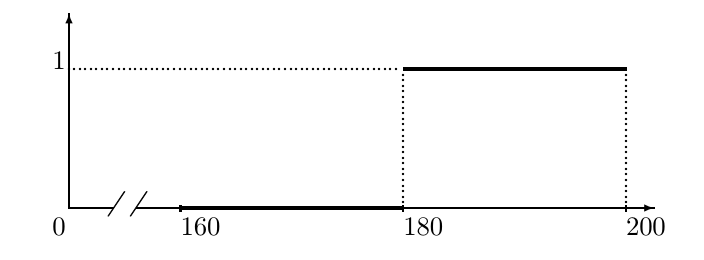
\includegraphics[width=100mm]{Images/Fig1.png}
	\caption{تابع عضویت افراد قد بلند در مجموعه‌های کلاسیک}\label{fig:f_1}
\end{figure}
حال همین مثال را در مجموعه‌های فازی تعریف می‌کنیم. 
\end{exmp}
%##################################################################
 \subsection{ مفاهیم پایه مجموعه‌های فازی}
 \subsection{ روابط بین مجموعه‌های فازی}
 \subsection{عملیات بر روی مجموعه‌های فازی}
 \subsection{‌اعداد فازی}
  \subsubsection{ ‌اعداد فازی قطعه به قطعه درجه دوم}
  \subsubsection{‌اعداد فازی مثلثی}
  \subsubsection{‌اعداد فازی ذوزنقه‌ای}
 \subsection{رابطه‌های فازی}
 \subsection{عملیات بر روی رابطه‌های فازی}
%********************************Fuzzy Logic************************
\section{منطق فازی}
%********************************Other Sctions***********************
\section{کاربرد میانگین فازی برای پیش‌بینی}
\section{تصمیم‌گیری در محیط فازی}
\section{کاربرد کنترل فازی}
\section{مفاهیم اولیه هوش مصنوعی}
\section{جستجوی آگاهانه و ناآگاهانه}
%*******************************References**************************
\bibliographystyle{ieeetr-fa}
\bibliography{Ref}
\end{document}